\documentclass{standalone}

\usepackage{tikz}
\usepackage{standalone}
\usetikzlibrary{calc}

\begin{document}

    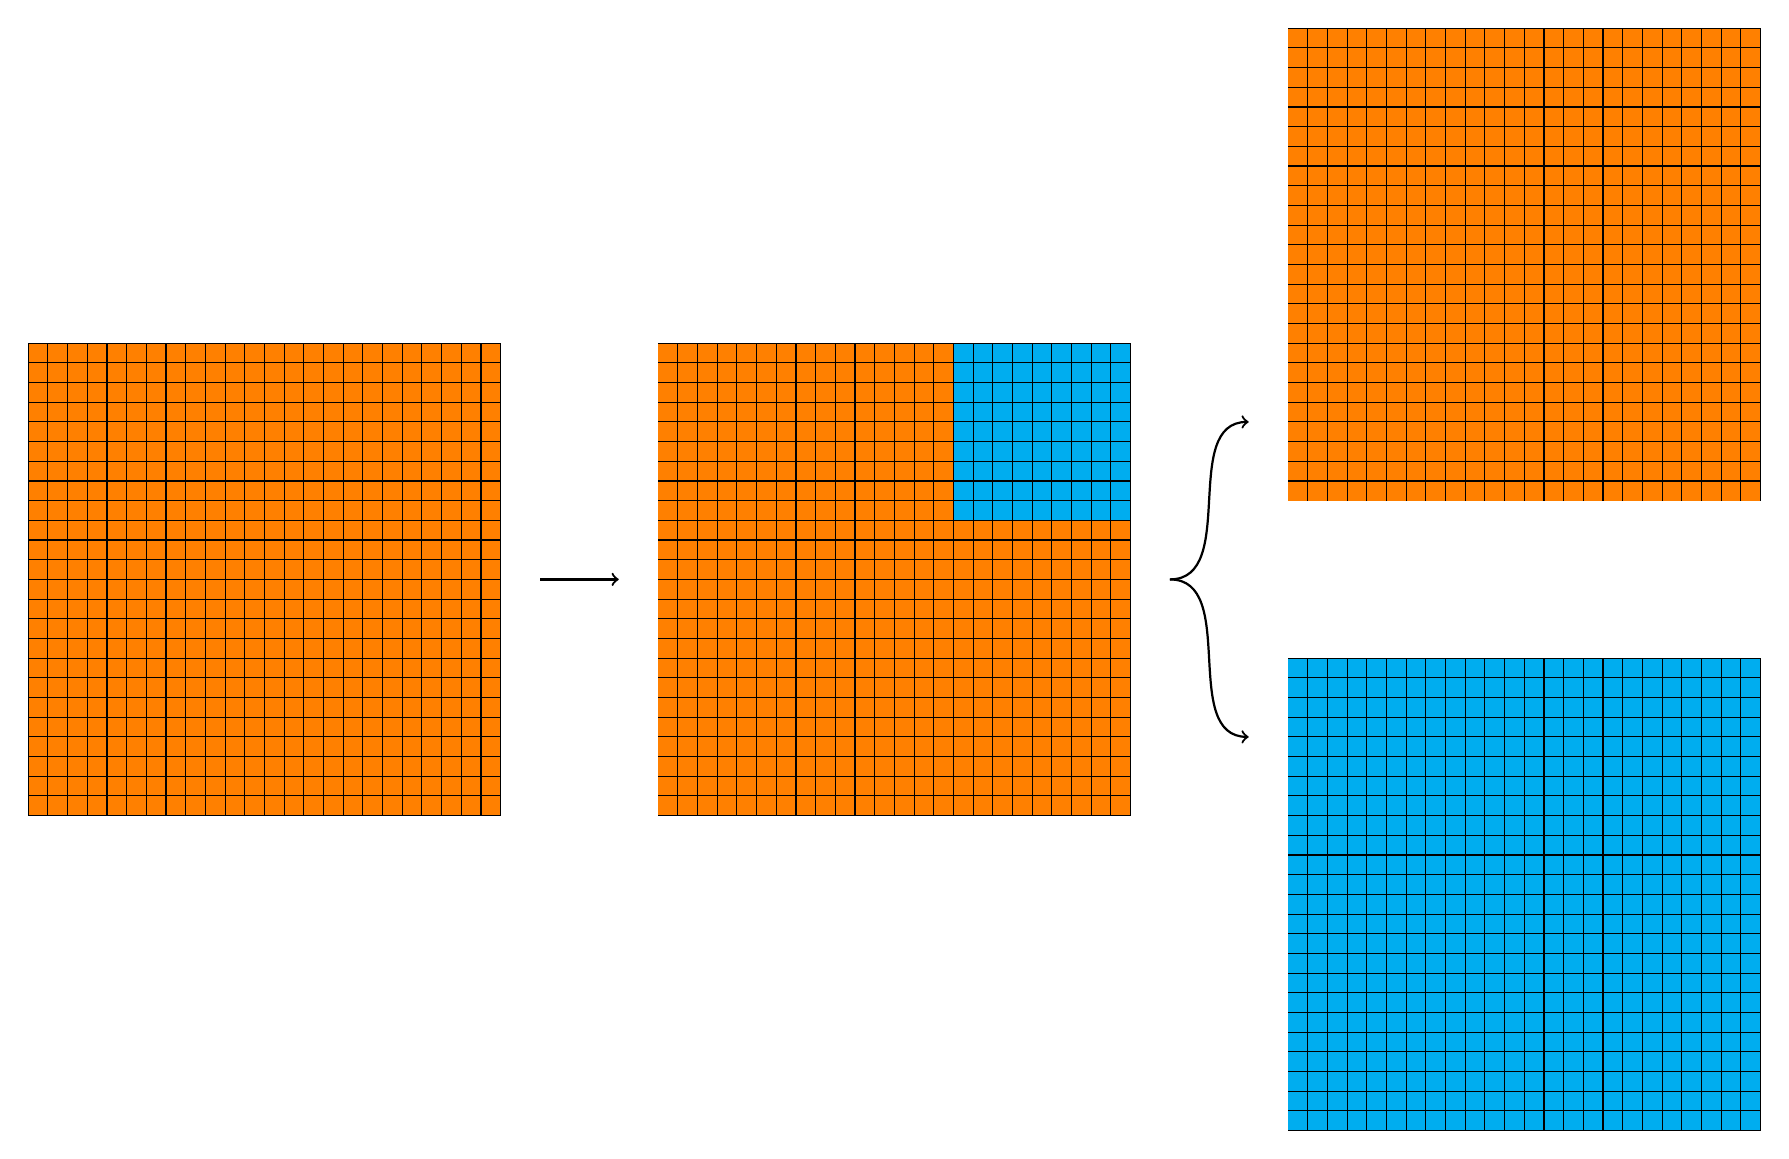
\begin{tikzpicture}

        \fill[orange] (0, 0) rectangle (6, 6);
        \draw[step=0.25cm, black] (0, 0) grid (6, 6);

        \draw (6.5, 3) edge[out=0, in=-180, ->, thick] (7.5, 3);

        \fill[orange] (8, 0) rectangle (14, 6);
        \fill[cyan] (11.75, 3.75) rectangle (14, 6);
        \draw[step=0.25cm, black] (8, 0) grid (14, 6);

        \draw (14.5, 3) edge[out=0, in=-180, ->, thick] (15.5, 5);
        \draw (14.5, 3) edge[out=0, in=-180, ->, thick] (15.5, 1);


        \fill[cyan] (16,-4) rectangle (22, 2);
        \draw[step=0.25cm, black] (16, -4) grid (22, 2);

        \fill[orange] (16, 4) rectangle (22, 10);
        \draw[step=0.25cm, black] (16, 4) grid (22, 10);


    \end{tikzpicture}

\end{document}